\documentclass{article}

\usepackage[utf8]{inputenc}
\usepackage[ngerman]{babel}
\usepackage[ngerman]{translator}
\usepackage[T1]{fontenc}
\usepackage{enumitem}
\usepackage{graphicx}
\usepackage{geometry}
\usepackage{float}
\usepackage{url}
\usepackage[bottom]{footmisc}
\usepackage{hyperref}
\usepackage[nonumberlist, section=subsection]{glossaries}
\usepackage{tabularx}

\usepackage{pifont}
\newcommand{\cmark}{\ding{51}}

\title{\textbf{Validierungsphase} \\ Cryptographics}
\author{}
\date{\today}

%Glossar-Befehle anschalten
\makeglossaries
% \newglossaryentry{identifier}{name={Name}, description={Description}}

\begin{document}

% The cover page.
\maketitle
\begin{table}[b]
  \begin{tabular}{| l | l | l |}
    \hline
    \textbf{Phase} & \textbf{Verantwortlicher} & \textbf{Email} \\ \hline
    Pflichtenheft & Matthias Jaenicke & matthias.jaenicke@student.kit.edu \\ \hline
    Entwurf & Matthias Plappert & undkc@student.kit.edu \\
            & Julien Duman & uncyc@student.kit.edu \\ \hline
    Implementierung & Christian Dreher & uaeef@student.kit.edu \\ \hline
    Qualitätssicherung & Wasilij Beskorovajnov & uajkm@student.kit.edu \\ \hline
    Präsentation & Aydin Tekin & aydin.tekin@student.kit.edu \\ \hline
    \end{tabular}
\end{table}
\thispagestyle{empty}
\newpage

% Table of contents page.
\tableofcontents
\newpage

% Start of the actual document.
\section{Einleitung}
 Die \textbf{Validierung} gestaltete sich ohne große Probleme. Es sind keine \textbf{schwerwiegenden} Fehler aufgetreten, die große Änderungen in der Programmlogik 
 erfordert haben. Da der \textbf{Entwurf und die Implementierung} sehr ausführlich gestaltet worden sind, konnte man \textbf{viele} Fehler bereits in ihrem Ursprung 
 ersticken bevor diese überhaupt auftreten konnten. Jedoch wurde bei der Implementierung die \textbf{Benutzerfreundlichkeit} vernachlässigt. Somit war
 dies das Leitthema bei der Validierung. Darauf wurde somit der größte Wert gelegt.\newline
 Die Fehler wurden alle bis auf ein paar \textbf{Ausnahmen} beseitigt und das Programm \textbf{benutzerfreundlicher} gestaltet. Die Verfahren wurden einheitlicher
 gemacht und unnötige, wie unintuitive UI-Elemente entfernt. Die Erklärungen wurden angepasst und das Layout marginal verändert.
\clearpage

\section{Testszenarien}
  Die folgenden Testszenarien sind bereits im Pflichtenheft im Kapitel 8 ``Testszenarien'' spezifiziert. Hier
  findet sich nur eine tabellarische Darstellnug derselben, um Funktionen, die im Fließtext beschrieben werden,
  einzeln verifizieren zu können.
  
  \subsection{Szenario 1}
    \begin{table}[H]
      \begin{tabularx}{\textwidth}{| >{\raggedright\arraybackslash}X | c |}
        \hline
        \textbf{Funktion} & \textbf{Erfüllt?} \\
        \hline
        Startbildschirm wird angezeigt & \cmark \\
        \hline
        Zeitleiste wird angezeigt & \cmark \\
        \hline
        Verfahren werden auf Zeitleiste dargestellt & \cmark \\
        \hline
        Verfahren sind farblich gekennzeichnet & \cmark \\
        \hline
        Caesar-Verfahren kann ausgewählt werden & \cmark \\
        \hline
        Popover mit Zusammenfassung wird dargestellt & \cmark \\
        \hline
        Verfahren kann gestartet werden & \cmark \\
        \hline
        Verfahren erlaubt mehrschrittige Navigation & \cmark \\
        \hline
        Verfahren enthält Einleitung & \cmark \\
        \hline
        Selbstversuch zur Verschlüsselung funktioniert & \cmark \\
        \hline
        Selbstversuch zur Entschlüsselung funktioniert & \cmark \\
        \hline
        Rückkehr zum Startbildschirm ist möglich & \cmark \\
        \hline
        Auswahl eines anderen Verfahrens ist möglich & \cmark \\
        \hline
        Am Ende des Verfahrens werden weitere Informationen sowie QR-Code dargestellt & \cmark \\
        \hline
        QR-Code enthält Link zu weiteren Informationen & \cmark \\
        \hline
      \end{tabularx}
    \end{table}

  \subsection{Szenario 2}
    \begin{table}[H]
      \begin{tabularx}{\textwidth}{| >{\raggedright\arraybackslash}X | c |}
        \hline
        \textbf{Funktion} & \textbf{Erfüllt?} \\
        \hline
        Zufällige Eingabe bringt das Programm nicht zum Abstürzen & \cmark \\
        \hline
        Verfahren kann ausgewählt werden & \cmark \\
        \hline
        Programm hat jederzeit einen Button um zum Startbildschirm zurückzukehren & \cmark \\
        \hline
      \end{tabularx}
    \end{table}

  \subsection{Szenario 3}
    \textit{Hinweis: Die Variablen x und y richten sich nach der aktuellen Konfiguration des Programmes. Hierbei
      ist x der Wert des Parameters \texttt{idleTimeout} sowie y der Wert des Parameters \texttt{resetTimeout}.}
    \newline

    \begin{table}[H]
      \begin{tabularx}{\textwidth}{| >{\raggedright\arraybackslash}X | c |}
        \hline
        \textbf{Funktion} & \textbf{Erfüllt?} \\
        \hline
        Verfahren kann ausgewählt werden & \cmark \\
        \hline
        Programm erkennt fehlende Eingabe nach x Sekunden & \cmark \\
        \hline
        Programm zeigt Warnhinweis, dass sich das Programm in y Sekunden zurücksetzen wird, dar & \cmark \\
        \hline
        Nach y Sekunden kehrt das Programm automatisch zum Startbildschirm zurück & \cmark \\
        \hline
      \end{tabularx}
    \end{table}

  \subsection{Szenario 4}

    \begin{table}[H]
      \begin{tabularx}{\textwidth}{| >{\raggedright\arraybackslash}X | c |}
        \hline
        \textbf{Funktion} & \textbf{Erfüllt?} \\
        \hline
        Programm läuft im Vollbildmodus & \cmark \\
        \hline
        Programm hat keine Möglichkeit um per Touchscreen-Eingabe zum Betriebssystem zurückzukehren & \cmark \\
        \hline
        Programm kann mithilfe einer angeschlossenen Hardwaretastatur beendet werden & \cmark \\
        \hline
      \end{tabularx}
    \end{table}
\clearpage

\section{Abdeckung der JUnit-Testfälle}
  Da Cryptographics vor allem aus GUI-Komponenten besteht, konzentrieren sich die JUnit-Testfälle auf die
  funktionalen Komponenten. Dies sind für die einzelnen Verfahren die Model-Klassen, welche die kryptographischen
  Funktionen bereit stellen. Im Paket CryptographicsLib wurden ebenfalls die Model-Klassen getestet sowie die Klasse
  AbstractVisualization, da diese grundlegender Bestandteil der gesamten Controller-Hierarchie ist.

  In allen genannten Klassen konnten immer wenigstens 80\% Abdeckung erreicht werden, in den meisten Fällen sogar
  weit über 90\%.

  \subsection{Paket edu.kit.iks.CryptographicsLib}
    \subsubsection{Klasse AbstractController}
      \begin{figure}[H]
        \centering
          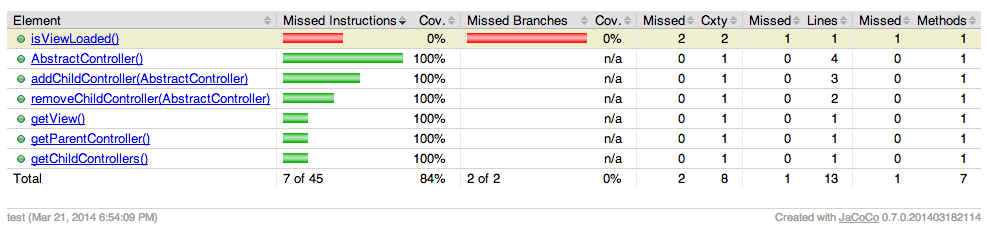
\includegraphics[width=\textwidth]{resources/coverage_lib_abstractcontroller}
      \end{figure}

    \subsubsection{Klasse Configuration}
      \begin{figure}[H]
        \centering
          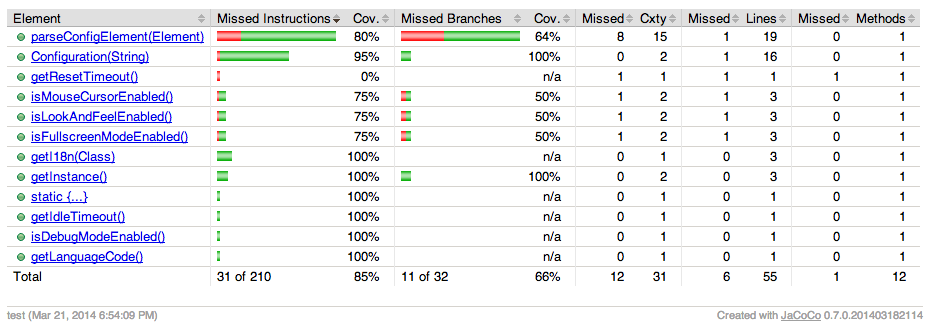
\includegraphics[width=\textwidth]{resources/coverage_lib_configuration}
      \end{figure}

    \subsubsection{Klasse VisualizationInfoLoader}
      \begin{figure}[H]
        \centering
          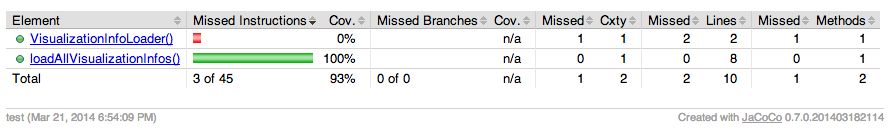
\includegraphics[width=\textwidth]{resources/coverage_lib_visualizationinfoloader}
      \end{figure}

  \subsection{Paket edu.kit.iks.Cryptographics.Caesar.Experiment}
    \subsubsection{Klasse CryptoModel}
      \begin{figure}[H]
        \centering
          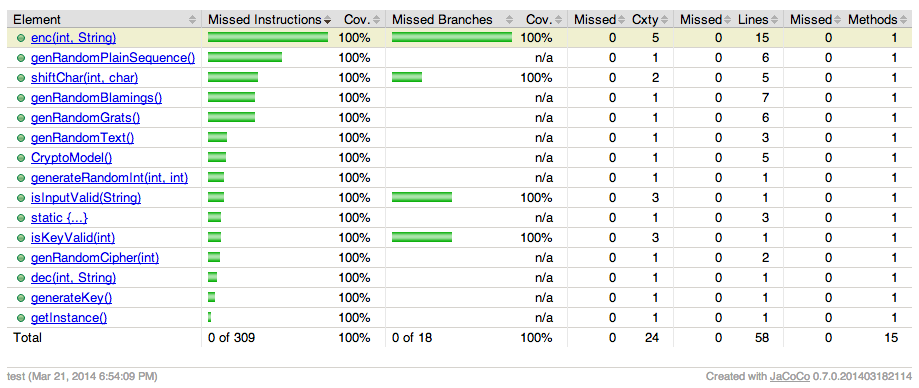
\includegraphics[width=\textwidth]{resources/coverage_caesar_model}
      \end{figure}

  \subsection{Paket edu.kit.iks.Cryptographics.DiffieHellman}
    \subsubsection{Klasse Model}
      \begin{figure}[H]
        \centering
          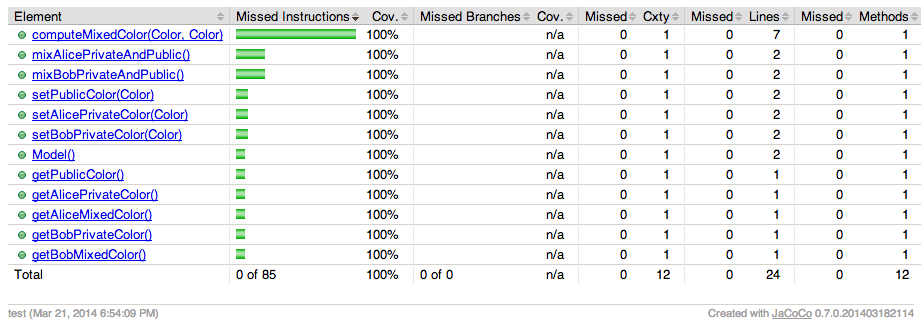
\includegraphics[width=\textwidth]{resources/coverage_diffiehellman_model}
      \end{figure}

  \subsection{Paket edu.kit.iks.Cryptographics.Vigenere}
    \subsubsection{VigenereModel}
      \begin{figure}[H]
        \centering
          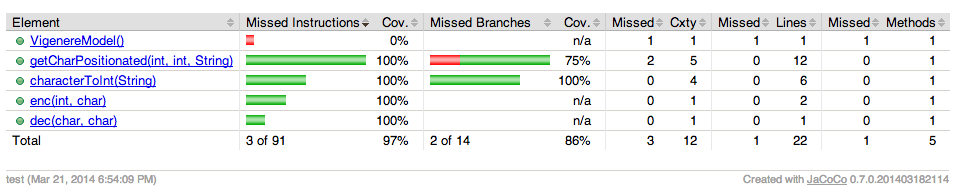
\includegraphics[width=\textwidth]{resources/coverage_vigenere_model}
      \end{figure}
\clearpage

\section{Regressionstests}
 \subsection{Caesar}
  \begin{enumerate}
   \item Leider konnte die UI nicht überall statisch gemacht werden. Beispielsweise bei der Demonstration der Caesar-Chiffre 
         Springt das alphabet wenn sich der untere Button ``Proceed'' mit der Tastatur abwechselt. Größenänderungen und Kapselung der 
         Alphabets hat zu keinem sinnvollen Ergebnis geführt. Die UI außerhalb der Demophase ist überall im Griff und es konnten 
         keine Sprüge mehr festgestellt werden.\newline 
         \textbf{Regressionstests für springende UI:}\newline
         Zu beachten ist, dass die Einführungsphase davon ausgeschlossen ist!\newline
         Gehe die Visualisierung des Verfahrens durch und achte auf UI-Elemente, die nach der Interaktion mit der Oberfläche 
         nicht an ihrem zugewiesenen Ort bleiben. Genauer:\newline
         1. Experiment: Beim entschlüsseln und entschlüsseln sollte alles statisch an seinem Ort bleiben und sich nichts bewegen.\newline
         2. Histogramme: Achte vor allem bei der Auswahl der Eingabebox für den Schlüssel, ob alles an seinem Ort bleibt, wenn die
            Tastatur erscheint.
   \item Überprüfe den ersten Schritt der Demonstration auf das Fehlen des Alphabets. Wenn er erst im 2ten Schritt erscheint, dann ist
         alles richtig.
   \item Experiment, ``Brute Force''-Phase: Probiere alle Schlüssel durch und wenn der richtige gefunden wird, drücke nochmals auf +1 oder -1
         und überprüfe ob die Grenzen des Kastens sich wieder blau gefärbt haben. Überprüfe auch ob sich die Anzeige an der oberen Kante
         des Kastens wieder anzeigt, dass der Schlüssel falsch ist.     
  \end{enumerate}

  \subsection{Diffie-Hellman}
  \begin{enumerate}
      \item Da der meiste Code sich um die grafische Oberfläche kümmert, ist es schwierig
          automatische Regressionstests zu schreiben, daher wurden manuelle Tests durchgeführt.
          Nach jeder Behebung eines Fehlers wurde das komplette Verfahren mehrmals durchgegangen.
          Dabei wurde drauf geachtet, das allen UI-Elemente weiterhin genug Platz eingeräumt wurde.

          Beispielexperiment 1:
          Überspringe die Einführung und Demonstration, gehe direkt zum Experiment.
          Wähle eine öffentliche Farbe und schicke diese an Bob.
          Wähle eine private Farbe und mische die Farben. Schicke eine falsche
          Farbe an Bob. Dabei wird drauf geachtet das der richtige Text, richtig positioniert
          erscheint, der dem Nutzer sagt, dass er eine falsche Farbe gewählt hat.

          Wähle jetzt die richtige Farbe und schicke sie an Bob.
          Klicke den Hilfe-Button um einen Tip zu bekommen.
          
          Klicke den Weiter-Button, damit Bob seine Mixtur an Alice sendet.
          Mische die Farben zum finalen Geheimnis, und komme auf den Informationsbildschirm.

          Beispielexperiment 2:
          Überspringe die Einführung und führe die Demonstration aus.
          Klicke dich durch die Demonstration, entscheide dich dafür
          nochmal dir die Einführung anzuschauen. Klicke dich zur Demonstration.
          Entscheide dich doch das Caesar-Verfahren anzuschauen statt Diffie-Hellman.
      \end{enumerate}
\clearpage

\section{Beschreibung der Fehler}
  Die meisten Bugs kamen aus der Sparte \textbf{Usability}. Vieles war in der Implementierungsphase nicht zu entdecken, da man damit beschäftigt
  war die UI überhaupt zum funktionieren zu bringen. Die meisten Schwierigkeiten machte da der \textbf{Layoutmanager}, der für uns oft nicht
  nachvollziehbare Reaktionen auf die Auslegung unsere UI-Elemente zeigte.\newline 
  Dies erschwerte beträchtlich die Auslegung einer \textbf{benutzerfreundlichen UI} und führte zu vielen Mängel, die man
  nur sehr spät entdeckt hatte. Somit sind in der Qualitätssicherung hauptsächlich usability Bugs ausgebessert worden. 
  Man hat Feedback zur UI unter anderem auch von unabhängigen Personen herangezogen und sich anhand dessen orientiert. 
  
  \subsection{Usability Bugs}
    \subsubsection{Caesar}
     \begin{enumerate}
      \item Das größte Problem bei der Caesar-UI waren die \textbf{springenden} UI-Elemente, die an ihrem ursprünglichen Ort hätten bleiben sollen.
            Wenn allerdings ein neues UI-Element erschienen ist oder ein alter verschwunden, beispielweise ein Button, dann hat der Layoutmanager kurzerhand auch alle anderen
            Elemente nach seinem Belieben ausgerichet. Dies führte oft zu zufälligen Ergebnissen, die nicht nachvollzierbar waren. Manchmal sogar nicht reproduzierbar.
            Nichtsdestotrotz konnte man nicht alle Fehler dieser Art beseitigen, da man den Ursprung nicht finden konnte.\newline 
            Es wäre zwar möglich die UI von einem anderen Layoutmanager auslegen zu lassen, jedoch hätte das den Zeitrahmen gesprengt, da die UI
            auf den \textbf{GridBagLayoutManager} ausgerichtet war. Das hätte ein völliges Neuschreiben der UI bedeutet. 
            
      \item Auch ein Problem waren die \textbf{Erklärungen}. Es hat sich herausgestellt, dass diese größtenteils sehr {unintuitiv} waren.
            Viele der Testpersonen haben sehr große Schwierigkeiten gehabt, da die Texte anfangs größer waren und eine kleinere Schrift hatten.
            Das erzeugte viel Mühseligkeit und war alles andere als \textbf{benutzerfreundlich}.\newline
            Auch wenn das nix zur Logik des Programms beigetragen hat, so hat es die \textbf{Benutzerfreundlichkeit} erheblich verbessert. 
            Schriftart wurde größer gesetzt und die Zeichen dick dargestellt, damit diese die \textbf{Aufmerksamkeit} des Users als erste auffangen.
            
      \item Viele \textbf{Unklarheiten} kamen mit der UI einher. Vor allem die Funktionalität mancher UI-Elemente war nicht auf einen Blick ersichtlich.
            Das erschwerte die Visualisierung, da der User die meiste Zeit damit beschäftigt war sich mit der UI rumzuschlagen. Es bestand die Gefahr, dass
            der Inhalt der UI in den Hintergrund gerückt wird und bei dem User \textbf{Frust} aufkommen könnte.\newline
            Das beste Beispiel war das \textbf{Alphabet} in der Demonstration des Verfahrens. Siehe Anhang \textbf{Caesar Demonstration}.\newline
            Der Sinn dessen war für den User nicht ersichtlich.
            So kam es dazu, dass der User versucht hat vergeblich das Alphabet \textbf{anzuklicken}. Dies führte zu \textbf{Irritationen}. Folgedessen wurde das Alphabet 
            in der Demonstration \textbf{entfernt}.\newline
            
            Ein anderes Beispiel ist das ``Brute Force'' Experiment. Siehe im \textbf{Anhang} unter ``Brute Force Experiment''.\newline
            
            Dieses leidete unter \textbf{mehreren} Mängeln. Die \textbf{ganze} UI war irritierend und unintuitiv.
            Viele der Testpersonen waren damit deutlich überfordert. Selbst die Erklärungen haben nicht deutlich machen können, was zu tun ist. 
            Man musste sich vieles selbst zusammenreimen. Die ganze UI wurde dann unter Usablity-Bugs eingestuft und musste überarbeitet werden.
            \begin{itemize}
             \item Als erstes wurde die \textbf{Farbe} des ``brute force'' Kastens zu \textbf{blau} umgestellt. Dies dient der Einheitlichkeit, da die ganze UI einen blauen 
                   Ton hat. Mehrere Testpersonen haben positiv drauf reagiert.
             
             \item Die eigentliche Erklärung der ``brute force'' Methode wurde in den Kasten verlagert. Und eine andere Erklärung drunter um die die Bedeutung
                   des Buttons zur den Histogrammen zu verdeutlichen. Früher stand dieser ohne viel Erklärung rum und führte zu vielen Beschwerden.
                   
             \item Der Button, der zu den Histogrammen führt wurde ganz nach unten verlagert, damit er die \textbf{Aufmerksamkeit} nicht fängt.
% 
             \item Ein letztes großes Problem dieses Experiments war, dass beim Finden des richtigen Schlüssels der Kasten \textbf{grün blieb} und die Glückwunsch Meldung
                   \textbf{nicht verschwand} auch wenn man weitere Schlüssel durchprobiert habe. Dies führte dazu, dass der User in vielen Fällen einen \textbf{Fehler} im Programm
                   angenommen hat. Dies wurde ausgebessert, sodass sich die Meldungen und der Kanten des Kastens dem aktuellen Schlüssel anpassen.
            \end{itemize}
     \end{enumerate}

     \subsubsection{Diffie-Hellman}
     \begin{enumerate}
         \item Beim Diffie-Hellman Verfahren, gab es mehrere unintuitive Bedienungselemente, welche behoben worden sind.
             Dazu gehört dass es dem Nutzer beim Experiment unklar sein könnte, wessen Farben er mischen soll,
             da die Farben die ausgewählt werden, neben Bob dargestellt wurden. Siehe \textbf{Anhang} unter ``Diffie-Hellman Experiment''.\newline
             
             Jetzt werden die Farben,
             die man auswählen und mischen soll, neben Alice dargestellt. Somit sollte klarer sein wessen Rolle
             der Nutzer einnimmt.
             Es wird zwar im erklärenden Text erwähnt wessen Rolle der Nutzer einnimmt, aber durch die Positionierung
             wird dies noch klarer.
         \item Ein weiterer Fehler war, dass sich Farbkreise im Farbkanal überlappt haben,
             was dadurch verursacht wurde, dass der Layoutmanager dem Farbkanal-JPanel zu wenig Platz eingeräumt hat.
             Dies war leicht zu beheben, indem man die Gewichte (in den GridBagConstraints) erhöht,
             und somit diesem JPanel mehr Platz einräumt.
         \item Ein weiteres Problem war, dass bei den Unterschiedlichen Farben die dargestellt wurden,
             man schnell die Übersicht verloren hat, insbesonderer wenn man das Verfahren könnt. Siehe das Problem und die Lösung \textbf{Anhang} ``Diffie-Hellman Experiment''.
             Um dies zu beheben haben wir die Farben mit Abkürzungen annotiert und eine Legende hinzugefügt,
             die erklärt welche Farbe was ist.
         \item Das größte Usability Problem war allerdings dass Buttons gesprungen sind.
             Dies wurde durch ein JLabel verursacht, welches seine Größe geändert hat,
             wenn man den Text mit der setText() Methode geändert hat.
             Dadurch wurde vom LayoutManager die aktuelle View repositioniert, was die springende Buttons
             zu folge hatte.
             Gelöst wurde dies, indem wir mit HTML die Größe spezifiziert haben, wodurch die Größe konstant bleibt,
             und somit keine Repositionierung stattfindet.
     \end{enumerate}

     \subsection{Funktionalitätsfehler}
     \subsubsection{Diffie-Hellman}
     \begin{enumerate}
         \item Da das Verfahren sehr simpel ist, haben wir nur einen Fehler entdeckt.
             Dieser war allerdings nicht ein Fehler vom Verfahren selbst, sondern
             ein kleiner Fehler vom Rahmenwerk. Der Fehler war, dass Timer vom DH-Verfahren weiterliefen,
             wenn man den Exit-Button geklickt hat. Da das Rahmenwerk die Kontrolle über diesen Button
             hat, ist es die Aufgabe des Exit-Button-Handler eine Methode vom Verfahren aufzurufen,
             um dem Verfahren die Chance zu geben sich sauber zu beenden. Dies wurde
             durch einen einfachen Einzeiler korrigiert. Es muss nur die unloadView() Methode der aktuellen
             View des Verfahrens aufgerufen werden.
             Da nur beim Diffie-Hellman Verfahren Timer verwendet wurden, ist dieser
             Fehler bei den anderen Verfahren nicht aufgetreten.
         \end{enumerate}

    \subsubsection{InformationController}
     \begin{enumerate}
         \item Der Status des Scroll-Down-Buttons war bei kurzen Texten fälschlicherweise auf aktiv gesetzt
         und wurde erst nach dem Anklicken korrekt aktualisiert. Das Problem wurde behoben.
         \end{enumerate}
\clearpage

% We may need this, or not...
\section{Anhang}
 \subsection{Caesar}
  \subsubsection{Brute Force Experiment}
   \begin{itemize}
    \item Alte Version des ``Brute Force'' Experiments und die sichtbaren Usability Probleme.\newline
          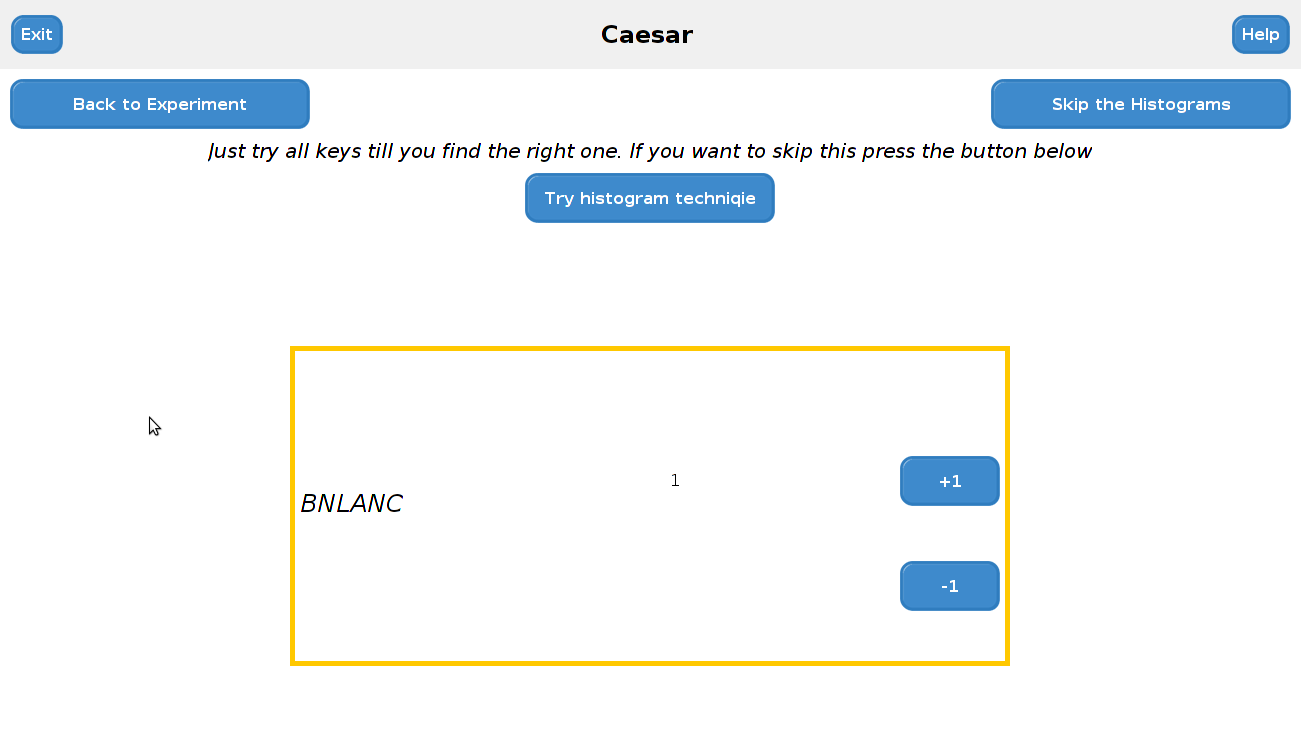
\includegraphics[width=15cm]{resources/bruteForceUsability.png}
    \newpage
    \item Neue Version des Experiments ``Brute Force''.\newline
          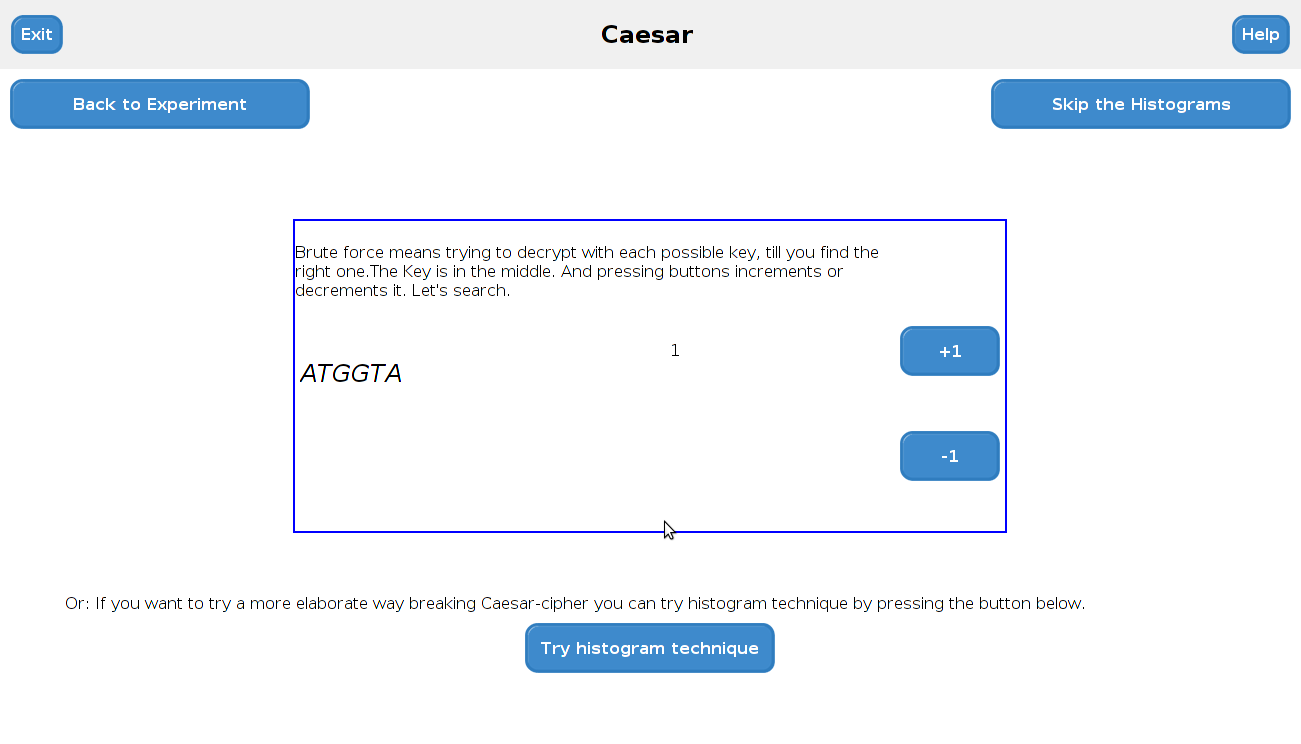
\includegraphics[width=15cm]{resources/bruteForceFix.png}
   \end{itemize}
   \subsubsection{Caesar Demonstration}
    \begin{itemize}
     \item Man sieht hier deutlich, dass das Alphabet unnötig ist und zur Verwirrung führen kann.\newline
           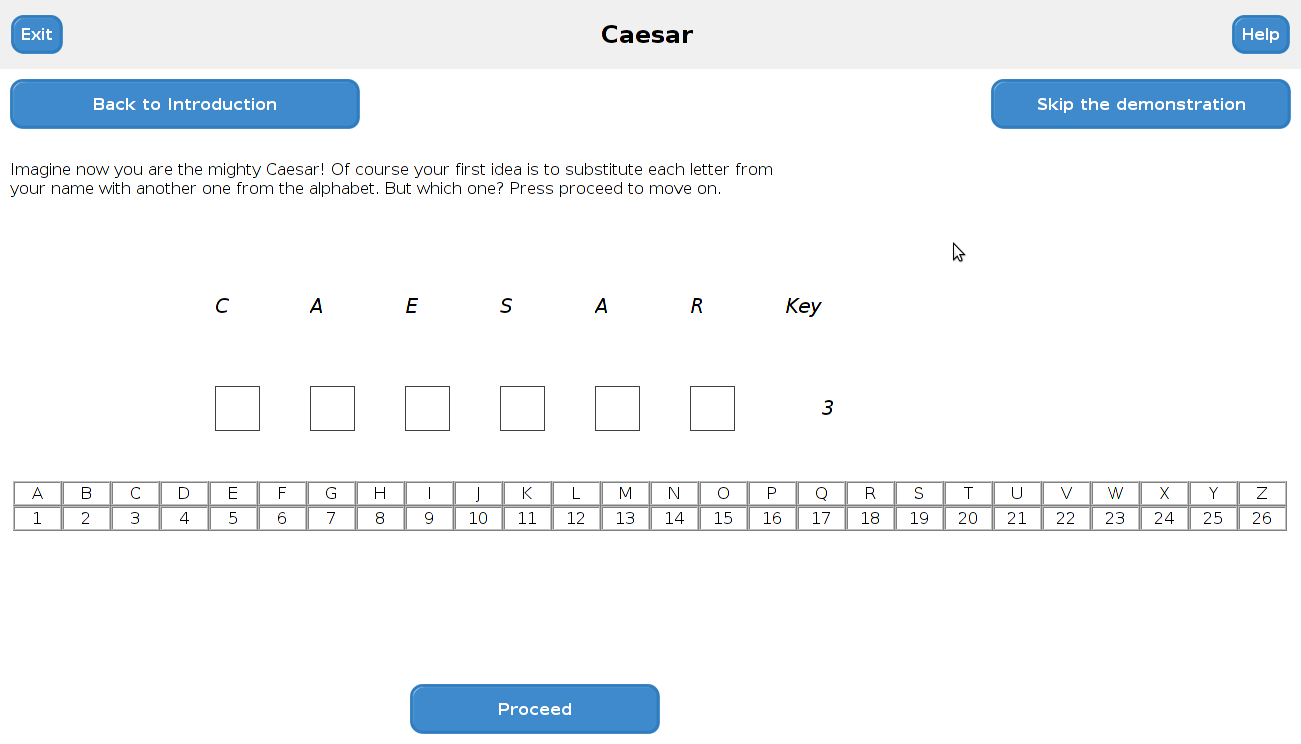
\includegraphics[width=15cm]{resources/caesarDemoUsability.png}
    \end{itemize}
   \subsection{Diffie-Hellman}
    \subsubsection{Diffie-Hellman Experiment}
     \begin{itemize}
      \item Die Sicht auf die alte UI des Experiments in Diffie-Hellman.\newline
            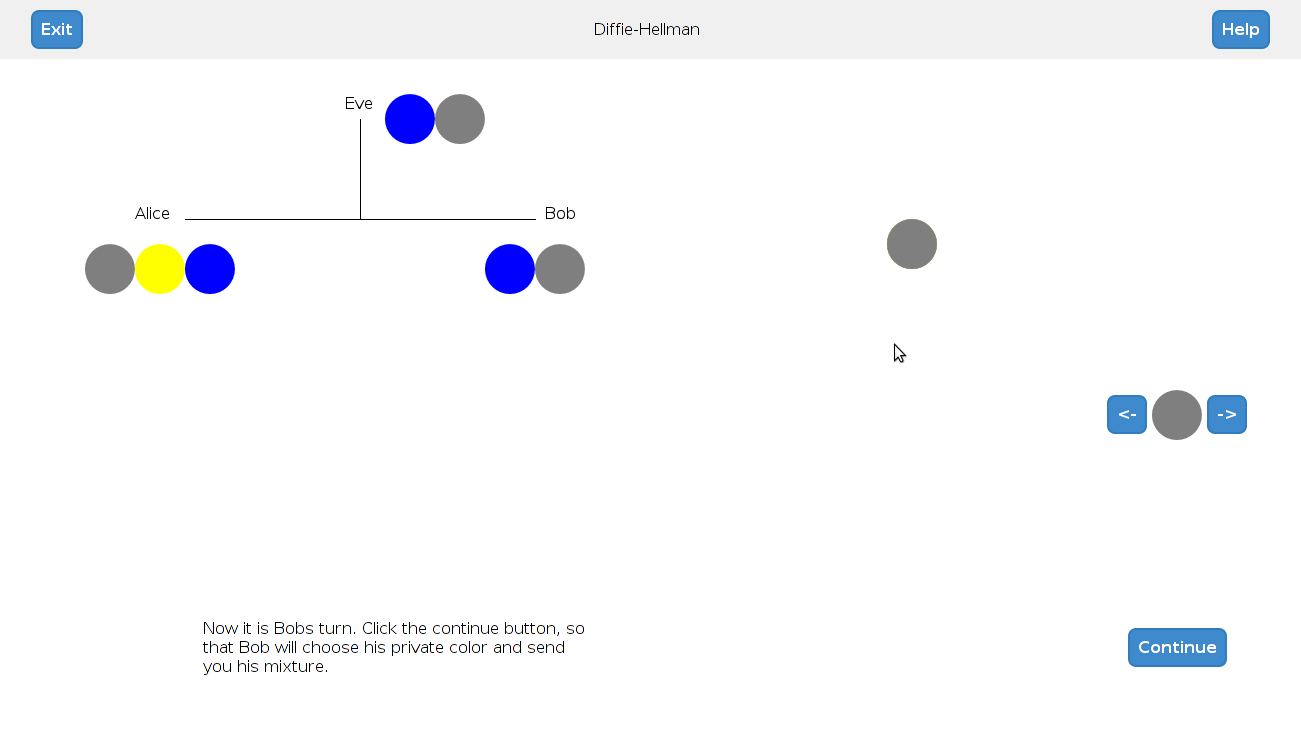
\includegraphics[width=15cm]{resources/dhExperiment.png}
      \newpage
      \item Die aktuelle Sicht auf die UI des Experiments in Diffie-Hellman\newline
            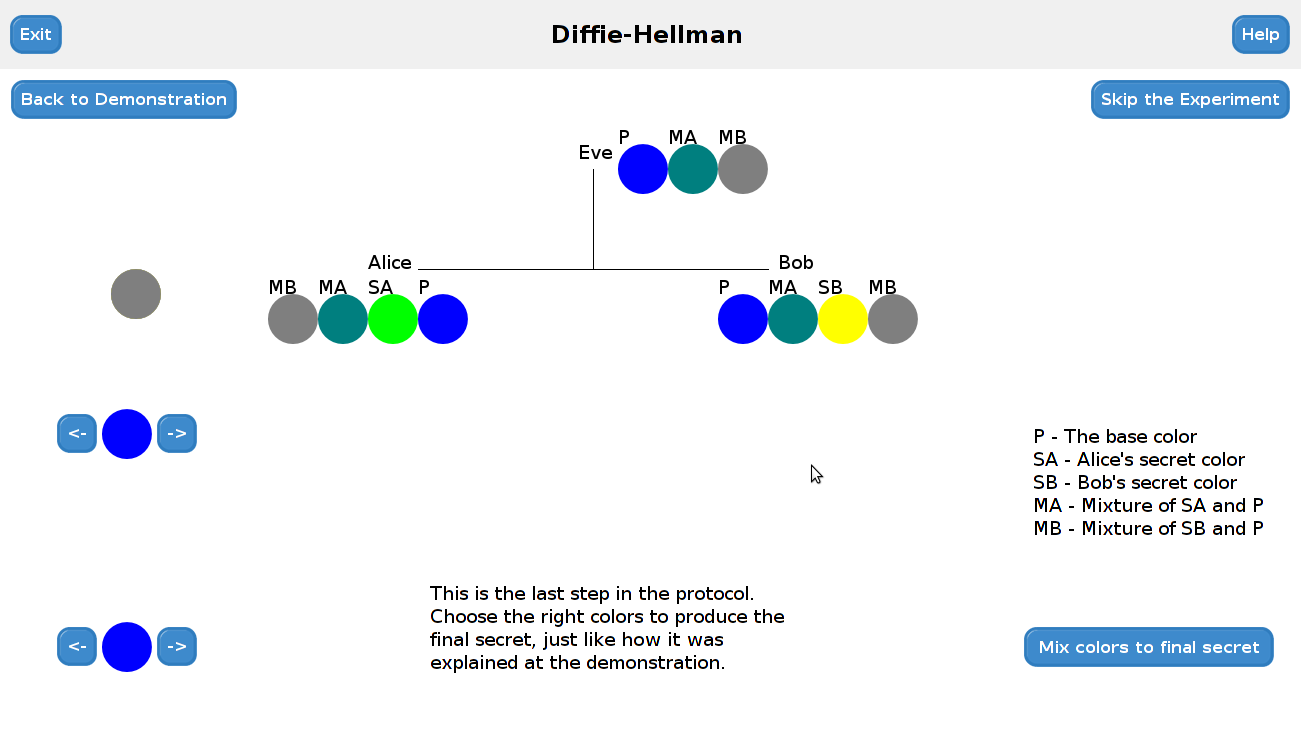
\includegraphics[width=15cm]{resources/dhUsabilityFix.png}
     \end{itemize}
    
    
\section{Glossar}

 \restoregeometry

\glsaddall
\printglossary[numberedsection, style=altlist]

\end{document}
